\documentclass[useAMS,usenatbib]{mn2e}
\usepackage{graphicx}
\newcommand{\figpath}{./Figs/}

% If your system does not have the AMS fonts version 2.0 installed, then
% remove the useAMS option.
%
% useAMS allows you to obtain upright Greek characters.
% e.g. \umu, \upi etc.  See the section on "Upright Greek characters" in
% this guide for further information.
%
% If you are using AMS 2.0 fonts, bold math letters/symbols are available
% at a larger range of sizes for NFSS release 1 and 2 (using \boldmath or
% preferably \bmath).
%
% The usenatbib command allows the use of Patrick Daly's natbib.sty for
% cross-referencing.
%
% If you wish to typeset the paper in Times font (if you do not have the
% PostScript Type 1 Computer Modern fonts you will need to do this to get
% smoother fonts in a PDF file) then uncomment the next line
% \usepackage{Times}

%%%%% AUTHORS - PLACE YOUR OWN MACROS HERE %%%%%


%%%%%%%%%%%%%%%%%%%%%%%%%%%%%%%%%%%%%%%%%%%%%%%%



\title[Geometrically thin acrretion disk around white dwarfs and quark stars]{Geometrically thin acrretion disk around white dwarfs and quark stars}
\author[B. Mishra, B. Vaidya and W. Kluzniak]{B. Mishra$^{1}$\thanks{E-mail:
mbhupe@camk.edu.pl}, W. Klu\'zniak$^{1}$, B. Vaidya$^{2}$\\
$^{1}$Copernicus Astronomical Center, Bartycka 18, Warsaw,00-716, Poland\\
$^{2}$University of Leeds, Leeds LS2 9JT, United Kingdom}
\begin{document}



\date{Accepted *** Received ***}

\pagerange{\pageref{firstpage}--\pageref{lastpage}} \pubyear{2014}

\maketitle

\label{firstpage}

\begin{abstract}
We studied semi-analytically and numerically the geometrically thin and optically thick accretion disk around rapidly rotating quark stars and white dwarfs using potential for Maclaurin spheroid. The main interest is to investigate the inner region of the so called $\alpha$-disk. We found that the change in eccentricity of the compact object influence the spectra emitted from the accretion disk. This can be observational evidence for the existance of the quark stars. Analytical calculations are mainly done in the radiation pressure dominated region of the accretion disk. The numerical work has been carried out to see the time evolution of the accretion disk around quark stars and white dwarfs using the same potential for Maclaurin spheroids. We showed that if the eccentricity of the object is high the matter will diffuse slowly and advect rapidly during its evolution. This gives a clue that how spin up or spin down can change the time evolution of the accretion disk using a very simple Newtonian approach.  

\end{abstract}

\begin{keywords}
Maclaurin spheroids, white dwarfs, quark stars, accretion disk
\end{keywords}

\section{Introduction}

\section{Physical Model}
\subsection{MacLaurian Spheroid}
\begin{itemize}
\item Describe in very brief the basics and how $\Omega$ is obtained
  and re-draw the plot that is in your supervisor paper. 
\end{itemize}
In general the accretion disk has been studied for the spherical potential which corresponds to Keplerian velocity. We are using potential for the Maclaurin spheroids which corresponds to angular velocity which is non-Keplerian very close to surface of star. The detailed description of the angular velocity has been studied by Kluzniak et al 2013. The angular velocity on the equatorial plane at a radial distance $r$ from the center of Spheroidal quark star with eccentricity $e$ semi-major axis $a$ is given by Eqn.1
\begin{figure}
\centering
\includegraphics[width=1\columnwidth]{\figpath/angular.eps}
\caption{Angular velocity distribution for chosen Maclaurin spheroid potential}
\label{fig:steadyplt1}
\end{figure}
\begin{equation}
\Omega ^2 \left(R\right)= 2\pi G\rho_* \frac{(1-e^2)^{1/2}}{e^3}\left[\gamma - \cos \gamma \sin\gamma \right]
\end{equation}  
where $\gamma = \arcsin (\frac{a e}{r})$ and $\rho *$ is density of star.
The disk structure will be defined by the angular momentum equation (SS-1973, Eqn.(2.2)),
\subsection{Steady thin accretion disk}
\begin{itemize}
\item List all the equations that you have used and what modification
  you have done for e.g., you have used $\Omega$ corresponding to
  MacLaurian spheroid. 
\item Say that formulae depends on M, Mdot, $\alpha$, r and
  eccentricity and give the values of choices made for them. 
  Explicit formulae and quantities shall be discussed in results
  section.
\end{itemize}
Now we can use Eqn.1 and follow exactly same steps as Shakura Sunyaev 1973, we shall arrive at three different regions of the disk. Our main concern here will be inner region, which is radiation pressure dominated region. We shall present all the equations and algebraic parameters in the second and third regions also but since we know that at large radii our results reduce to Newtonian results we shall describe inner region in more detail.
\subsubsection{Radiation pressure dominated region}
Shakura Sunyaev 1973 considered three different regions in the accretion disk, the inner one is radiation pressure dominated where in the interaction of matter and radiation electron scattering on free electrons has dominating contribution. Fig.x1 confirms that our results are in the region where radiation pressure is dominated over the gas pressure. We shall directly write the final form of the algebraic equations to calculate the different parameters in the disk. A detailed step by step calculation has been added in the appendix. Appendix also includes the algebraic equations for the gas pressure dominated regions.
\begin{equation}
z_0(r) = \frac{\sigma\rho_0\dot{M}k_1\left(p_1^{1/2}r^2 - p_2^{1/2}R_0^2\right)(ae)^3}{8\pi r^5 c \rho \Omega^2\cos\gamma(\gamma - \sin\gamma\cos\gamma)^{1/2}}.
\end{equation}
\begin{equation}
\Sigma(r) = \frac{32\pi c^2\rho^2 r^8 \cos^2{\gamma}(\gamma - \sin\gamma\cos\gamma)^2}{\alpha\sigma^2\rho_0^2 k_1^{1/2}(ae)^6\dot{M}\left(p_1^{1/2}r^2 - p_2^{1/2}R_0^2\right)}.
\end{equation}
\begin{equation}
\varepsilon(r) = \frac{6 r^3 c \cos\gamma(\gamma - \sin\gamma\cos\gamma)^{3/2}k_1^{1/2}}{\alpha\sigma (ae)^3}
\end{equation}
\begin{equation}
T(r) = \frac{6r^3 c \cos\gamma (\gamma - \sin\gamma\cos\gamma)^{3/2}k_1^{1/2}}{b^{1/4}\alpha\sigma (ae)^3}
\end{equation}
\begin{equation}
\tau (r) = \sqrt{\sigma_T(0.11 T^{-7/2}n)}\Sigma(r)
\end{equation}
\begin{equation}
n(r) = \frac{\Sigma(r)}{2mpz_0(r)}
\end{equation}
\begin{equation}
v_r(r) = \frac{\dot{M}}{2\pi\Sigma r}
\end{equation}
where, 
\begin{equation} 
\gamma = \arcsin(\frac{ae}{r}) 
\end{equation}
\begin{equation}
\gamma_0 = \arcsin(\frac{ae}{R_0})
\end{equation}
\begin{equation}
p_1 = (\gamma - \sin\gamma\cos\gamma)
\end{equation}
\begin{equation}
p_2 = (\gamma_0 - \sin\gamma_0\cos\gamma_0)
\end{equation}
$\dot{M}$ is mass accretion rate, $z_0(r)$ is half thickness of the disk, $\Sigma(r)$ is the radial distribution of surface density, $\varepsilon(r)$ is radial distribution of energy density, $T(r)$ is radial distribution of the temperature, $\tau(r)$ is opacity, $n(r)$ is the number density and $v_r$ is the radial velocity of the matter in the steady thin accretion disk.
\subsection{Non-stationary accretion disk}
\begin{itemize}
\item List formulae and refer the paper that we have been using for
  evolution of Surface density. 
\end{itemize}
The disk can not be stationary due to viscous forces acting to transport the angular momentum and cause the accretion of the matter. Here we numerically studied the time evolution of the thin accretion disk around quark stars. We shall integrate numerically the diffusion equation with constant viscosity. We adapted numerical scheme described in Brensteil et al 2010. For the potential we adapted from Maclaurin spheroids gives the different angular velocity profile so we shall write the diffusion equation in terms of angular velocity.
\begin{equation}
\frac{\partial\Sigma}{\partial t} = -\frac{1}{r}\frac{\partial}{\partial r}\left[\frac{1}{2\pi(r^2\Omega)^\prime}\frac{\partial G}{\partial r}\right]
\end{equation}
where,
\begin{equation}
G(r,t) = 2\pi r\nu\Sigma r^2 \Omega^\prime 
\end{equation}
Now if we choose the Keplerian angular velocity the above equations will reduce to standard diffusion equation used for study of disk evolution by various models based on $\alpha$-disk models.
\begin{equation}
\frac{\partial\Sigma}{\partial t} = \frac{3}{r}\frac{\partial}{\partial r}\left[r^{1/2}\frac{\partial}{\partial r}\left(\nu\Sigma r^{1/2}\right)\right]
\end{equation}
\begin{equation}
v_r = -\frac{3}{\Sigma r^{1/2}}\frac{\partial}{\partial r}\left(\nu\Sigma r^{1/2}\right)
\end{equation}
where $\Sigma$ is the surface density, $\nu$ is kinematic viscosity.

\section{Results}
\subsection{Steady state disk}
\begin{figure}
\centering
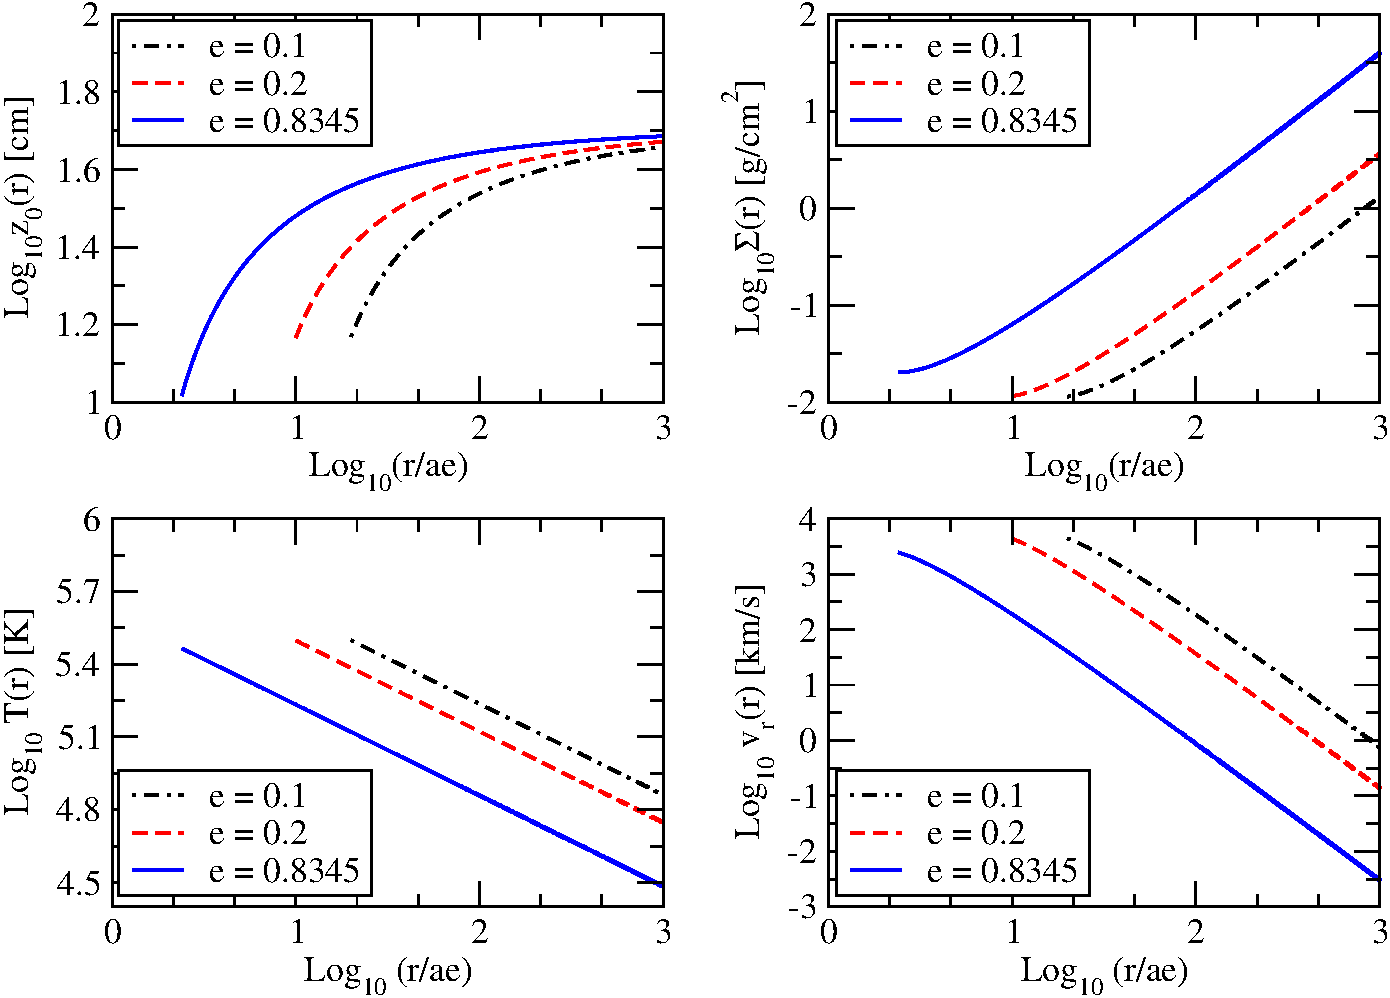
\includegraphics[width=1\columnwidth]{\figpath/multiplot_rho_alpha0001.pdf}
\caption{Multiplot of height, surface density, temperature and radial velocity variation with radial distance from the center of the star }
\label{fig:steadyplt1}
\end{figure}

\begin{itemize}
\item describe the multi plots (fig~\ref{fig:steadyplt1}) for each quantity : its value, its
  profile and dependence on eccentricity.
\item Make a table which gives quantitive values.  
\end{itemize}
\subsection{Disk thermodynamics and Spectra}
\begin{itemize}
\item Show that values of T obtained above give Prad $>$ Pgas. 
\item Also show that the disk is optically thick.
\item Finally describe the spectra and state its dependence on
  eccentricity. (Explain the reason in discussion).
\end{itemize}
\begin{figure}
\centering
\includegraphics[width=1\columnwidth]{\figpath/pradpgas.eps}
\caption{Plot shows the the inner region of investigation in which we assumed that radiation pressure dominates over gas pressure}
\label{fig:steadyplt1}
\end{figure}
\subsection{Evolution of surface density}
\begin{itemize}
\item Show the plot of evolution of a ring of matter for a particular high
  eccentricity and describe it. Specially the skewed profile for
  higher eccentricity. 
\item Show that at low eccentricity it approaches the $\alpha$-disk
  solution. Here also describe the plot which shows the evolution with
  different eccentricity. 
\end{itemize}
\begin{figure}
\centering
\includegraphics[width=1\columnwidth]{\figpath/nu1e-4.eps}
\caption{Time evolution of the ring of matter at a particular radius. Higher the eccentricity slower the evolution}
\label{fig:steadyplt1}
\end{figure}
\begin{figure}
\centering
\includegraphics[width=1\columnwidth]{\figpath/nu1e-4_05_0001.eps}
\caption{Time evolution of the accretion disk. Higher the eccentricity slower the evolution}
\label{fig:steadyplt1}
\end{figure}
\section{Discussion}
\subsection{Very thin and fast disk}
\begin{itemize}
\item Why few cm sized disk?
\item Is Newtonian gravity responsible for faster disk. 
\item how values change with change in $\alpha$. 
\end{itemize}

\subsection{Dependence of Spectra on eccentricity}
\begin{itemize}
\item Explain the reason for the dependence of spectra on e. 
\item Discuss its consequences in observations.
\end{itemize}

\subsection{Angular Momentum transport in disks}
\begin{itemize}
\item Explain the reason for skewness in sigma plot with high e
  values. Show plots of advection and diffusion. 
\item Also discuss the implication of e on Ang. momentum transport. 
\end{itemize}

\section{Conclusion}
State your conclusions here. 






\label{lastpage}
\end{document}
